\documentclass{scrartcl}
% Blaðsíðustillingar

\usepackage{geometry}

\geometry{
	paper=a4paper, % letterpaper lika til
	top=2.5cm, % Top margin
	bottom=1cm, % Bottom margin
	left=2.5cm, % Left margin
	right=2.4cm, % Right margin
	headheight=0.75cm, % Header height
	footskip=1.5cm, % Space from the bottom margin to the baseline of the footer
	headsep=0.75cm, % Space from the top margin to the baseline of the header
	%showframe, % Uncomment to show how the type block is set on the page
}

%-------------------------------- Íslenska ----------------------------
\usepackage[T1]{fontenc}
\usepackage[utf8]{inputenc}
%\usepackage[icelandic]{babel}

%----------------------------- Stærðfræðipakkar frá AMS ---------------

\usepackage{amsmath, amsfonts, amsthm, amssymb} % Stærðfræðipakkar
\usepackage{braket, nicefrac} % fyrir mengi, brotabrot

% ----------- Fyrir SI Einingar
\usepackage{siunitx}


%------------------------------ Listar/ númeringar -------------------------
\usepackage{enumitem, multicol}

%------------------------------- Fyrir innsetningu mynda --------------
\usepackage{graphicx, float} 
\usepackage{keystroke}
\usepackage{pgfplots}\usepgfplotslibrary{units}
\pgfplotsset{compat=1.18}

% ----------------- Til að teikna/tekka myndir -----------------------------
\usepackage{tikz}
\usepackage{tkz-euclide}
\usetikzlibrary{math}
\usepackage{fourier}
\usetikzlibrary{quotes,angles}
\usepackage{tkz-euclide}
\usetikzlibrary{calc}
%\usetkzobj{all}
\usepackage[siunitx]{circuitikz} %%<---Circuit Diagrams

%%%%%%%%%%%%%%%%%%%%%%%%%%
% Nýtt Matlab viðmót
\usepackage{listings}
\usepackage{fancyvrb}

\def\lstbasicfont{\fontfamily{pcr}\selectfont\normalsize}
\definecolor{mygreen}{RGB}{28,172,0} 
\definecolor{mylilas}{RGB}{170,55,241}
\lstset{language=Matlab,%
	basicstyle={\lstbasicfont},
	breaklines=true,%
	morekeywords={matlab2tikz},
	keywordstyle=\color{blue},%
	morekeywords=[2]{1}, keywordstyle=[2]{\color{black}},
	identifierstyle=\color{black},%
	stringstyle=\color{mylilas},
	commentstyle=\color{mygreen},%
	showstringspaces=false, %without this there will be a symbol in the places where there is a space
	numbers=left,%
	numberstyle={\tiny \color{black}},% size of the numbers
	numbersep=5 pt, % this defines how far the numbers are from the text 
	inputencoding=latin1,
	backgroundcolor = \color{gray!3},
	framexleftmargin= -1 mm,
	frame=none,
	rulesepcolor=\color{blue!30},
	extendedchars=true,
	emph={logical},emphstyle=\color{blue},	
	emph={all,equal, minor, on, off, long, short, bank, rat},emphstyle=\color{mylilas},	
}
\renewcommand\lstlistingname{\textsc{Matlab}}%

\usepackage{tcolorbox}
\tcbuselibrary{skins}
%Hérna vel ég stillingar fyrir ramma sem ég skýri matlabUT
\tcbset{matlabUT/.style={
		enhanced,
		colback=gray!1,
		colframe=gray!30,
		title=Command Window,
		arc=0mm,
		coltitle=black,
		center title, 
		title style={top color=white, bottom color = gray!30},
		grow to left by= -3 mm,
		left= 4 mm,
		grow to right by=0.5mm,
		colupper = gray!70!black
}}

% Les inn textaskra sem inniheldur niðurstöður úr Command Window
\newcommand{\CommandWindow}[1]{\begin{tcolorbox}[matlabUT]
		\VerbatimInput{#1}
\end{tcolorbox}}

%%%%%%%%%%%%%%%%    Matlab endar %%%%%%%%%%%%%%%%%%%%%%%%%%%%%%%%%%%%%%%%

% Formatta kóða

 \DefineVerbatimEnvironment%
      {verbatimprog}%
      {Verbatim}%
      {fontsize=\tiny}%

%%%%%%%%%%%%%%%%%%%%%%%%%% Hyperlink References %%%%%%%%%%%%%%%%%%%%%%%%%%%
\usepackage{hyperref}

%--------------------% Storage Path for images %-----------------%
\graphicspath{{graphics/}{Graphics/}{./}}
\usepackage[utf8]{inputenc}
\usepackage{enumerate}
\usepackage{relsize}
\usepackage{steinmetz}
\usepackage{verbatim}

\begin{document}

\begin{titlepage}
    \centering
    
\includegraphics[width=5cm]{RU_2.png}\par
    \vspace{1cm}
    {\scshape\LARGE Háskólinn í Reykjavík \par}
    \vspace{1cm}
    {\scshape\Large T-406-RAS2 \par}
	%\vspace{1.5cm}
    {\scshape\Large Circuit Design \par}
	\vspace{1.5cm}
	{\huge\bfseries Laboratory Exercise 3\par}
	\vspace{2cm}
	{\Large\itshape Björn Skarphéðinsson}\par
	\texttt{bjorns19@ru.is}\par
	\vspace{0.5cm}
	{\Large\itshape Eva María Hönnudóttir Sigurþórsdóttir}\par
	\texttt{eva19@ru.is}\par
	\vspace{0.5cm}
	{\Large\itshape Eyþór Mikael Eyþórsson}\par
	\texttt{eythore19@ru.is}\par
	\vfill
	Instructors:\par
	Slawomir Koziel \& Jón Hákon Richter

	\vspace{1cm}

% Bottom of the page
	{\large \today\par}
\end{titlepage}

\newpage
\tableofcontents

\section{Introduction}
\subsection{Scope}
The purpose of this exercise was to construct and measure the following low-pass filter circuits

\begin{enumerate}[a.)]
    \item Cascaded low-pass filter
    \item Sallen-key low-pass filter
\end{enumerate}

and observe the effects of varied impedance combinations on the output signal and it's quality factor.

\begin{figure}[H]
    \centering
        \begin{circuitikz} \draw
            (2,2.5) node[op amp] (opamp) {}
            (opamp.+) to [short] (0,2)
            to [short] (0,1)
            to node[ground] {} (0,1)
            (opamp.-) to [short, -*] (0,3)
            to [R, l=$R_1$, -o] (-2,3) node[left]{$v_s$}
            (0,3) to [short, -*] (0,4.5)
            to [short] (0,5.5)
            to [C, l=$C$] (3.5,5.5)
            to [short, -*] (3.5,4.5)
            to [R, l = $R_2$] (0,4.5)
            (3.5,5) to [short] (3.5,2.5)
            to [short] (opamp.out)
            (3.5,2.5) to [R, l=$R_1$, *-*] (6,2.5)
            (8,2) node[op amp] (opamp) {}
            (opamp.+) to [short] (6,1.5)
            to [short] (6,.5)
            to node[ground] {} (6,.5)
            (opamp.-) to [short] (6,2.5)
            to [short] (6,5)
            to [C, l=$C$] (9.5, 5)
            to [short, -*] (9.5, 4)
            to [R, l=$R_2$] (6, 4)
            (9.5, 4) to [short] (9.5,2)
            (opamp.out) to [short, -o] (10,2) node[right] {$v_o$}

        \end{circuitikz}
    \caption{Cascaded low-pass filter}
    \label{cascaded_circuit}
\end{figure}

\begin{figure}[H]
    \centering
        \begin{circuitikz}\draw
            (0,3) node[left] {$v_s$} to [R, l=$R_1$, o-*] (2,3)
            to [R, l=$R_2$, -*] (4,3)
            to [C, l=$C_2$] (4,1)
            to node[ground] {} (4,1)
            (2,3) to [short] (2,4.5)
            to [C, l=$C_1$] (8.5,4.5)
            to [short, -*] (8.5,2.5)
            to [short, -o] (9.5,2.5) node[right] {$v_o$}
            (7,2.5) node[op amp] (opamp) {}
            (opamp.-) to [short] (4,3)
            (opamp.+) to [short] (5.5,2)
            to [short] (5.5,1)
            to [short] (8.5,1)
            to [short] (8.5,2.5)
            (opamp.out) to [short] (8.5,2.5)
        \end{circuitikz}
    \caption{Sallen-key low-pass filter}
    \label{sallen_circuit}
\end{figure}
\subsection{Theory}
%Einföld útleiðsla á quality factor og útskýring á hvað það hann táknar

As their name suggests, low-pass filters are circuits that amplify low-frequency signals and dampen high frequency signals. Generally, the amplified bandwidth is called passband and the dampened bandwidth is the stopband. \newline

Ideally, the transition period between these bandwidths could be visualized as a straight vertical line and the total frequency response would resemble a step function, in reality however, the transition period varies with the order of the circuit and is represented by the dampening ratio

\begin{equation}
    \zeta = \frac{1}{2Q}
\end{equation}

where $Q$ is the quality factor describing the selectivity of the circuit. In some circuits, e.g. bandpass filters which have a definitive resonant frequency $\omega_0$, the quality factor is defined as

\begin{equation}
    Q = \frac{\omega_0}{B}
\end{equation}

in which case the bandwidth $B$ is the difference of the circuits half-power frequencies, hence describing the selectivity of the circuit. For our purposes this quality factor presents a selectivity about the cut-off frequency $\omega_c$, portraying qualities of resonance. 

\subsubsection{Cascaded Circuit}
%Útskýring og útleiðsla á cut-off frequency og quality factor f. Cascaded Circuit.



The transfer function of a low-pass filter is given by (note that for the cascaded filter $R_1 = R_2 = R$)
\begin{equation}
\label{lowpass_transfer}
    H(\omega_c) = \frac{1}{\sqrt{1+\omega_c^2R^2C^2}}
\end{equation}
A low-pass filter passes only the frequencies from dc up to the cutoff frequency, $\omega_c$. The cutoff frequency is where the transfer function's magnitude drops to $\frac{1}{\sqrt{2}} = 70.71\%$ of its maximum value. Thus, the cutoff frequency is obtained by setting the magnintude of the transfer function (eq. \ref{lowpass_transfer}) to $\frac{1}{\sqrt{2}}$.
\begin{equation*}
    H(\omega_c) = \frac{1}{\sqrt{1+\omega_c^2R^2C^2}} = \frac{1}{\sqrt{2}}
\end{equation*}
which yields
\begin{equation}
    \omega_c=\frac{1}{RC}
\end{equation}
Then the following equation is acquired to convert the cutoff frequency to Hz.
\begin{equation}
    f_c=\frac{\omega_c}{2\pi}
\end{equation}
The cutoff frequency is also the point where the power dissipated by the circuit is half of its maximum value.




\subsubsection{Sallen-key Circuit} % ----------------------------------------------------------------

The Sallen-key circuit is a unity gain low-pass filter, analogous to the second-order filter from Assignment 1. It's transfer function in terms of dampening factor $\zeta$ and cutoff frequency $\omega_c$

\begin{equation}
    H(s) = \frac{\omega_c^2}{s^2+2\zeta\omega_cs+\omega_c^2}
\end{equation}

displays a linear relationship of the dampening factor and s in the denominator

\begin{equation}
    2\zeta\omega_cs
\end{equation}

subsequently, the dampening factor affects the incline or 'sharpness' of the transition period between passband and stopband. In terms of quality factor Q the transfer function 

\begin{equation}
    H(s) = \frac{\omega_c^2}{s^2+\frac{\omega_cs}{Q}+\omega_c^2}
\end{equation}

displays an inverse relationship between Q and s in the denominator, consequently the quality factor affects the height and width of the peak frequency response. \\ \newline
%
Derivation of the transfer function for the circuit in figure (\ref{sallen_circuit}) yielded the cutoff frequency

\begin{equation}
    \omega_c=\frac{1}{\sqrt{R_1R_2C_1C_2}}
\end{equation}

and a quality factor of

\begin{equation}
    Q = \frac{\sqrt{R_1R_2C_1C_2}}{C_2(R_1+R_2)}.
\end{equation}

Notably, when circuit components fulfil

\begin{equation}
    R_1 = R_2, C_1 = C_2
\end{equation}

the cutoff frequency becomes

\begin{equation}
    \omega_c = \frac{1}{RC}
\end{equation}

and the quality factor

\begin{equation}
    Q = \frac{1}{2}
\end{equation}

\section{Method} % ---------------------------------------------------------------------------------
\subsection{Equipment \& Setup}
%Rás byggð á brauðbretti \newline
%DC $\pm$ 15V tengt í op amp \newline
%Probe-ar tengdir við input og output (taka fram hvaða channel er hvað) \newline
%MYND AF SETUP-I \newline

The elements of the circuits, as seen in fig.\ref{cascaded_circuit} and fig.\ref{sallen_circuit}, were inserted in a breadboard to build the circuits. A DC source was used to supply $\pm15 V$ to the LM741 op-amps. An oscilloscope was connected to the input and output of the circuits using probes in order to observe the signal.

%%Tókum við mynd af setupi???%%

\subsection{Procedure}
%AÐGERÐARRÖÐ \newline
%íhlutir mældir \newline
%rásir byggðar \newline
%mælingar teknar með oscilloscope \newline

For both circuits, the following order of operations was followed.\\
Each element of the circuit was measured (values of the elements stated in tables \ref{cascade_component_values} through \ref{sallen_component_values_20}) and then the circuit built (as depicted in fig. \ref{cascaded_circuit} and fig. \ref{sallen_circuit}) on the breadboard. Finally, the cut-off frequencies of the filters were measured using the oscilloscope.

Additionally, the Sallen-Key filter was redesigned to achieve certain ratios between the capacitors. The circuit was then rebuilt for each case and the cut-off frequencies measured again.

%%% það má alveg fikta í þessum töflum %%%
\begin{table}[H]
    \centering
    \begin{tabular}{|c|c|c|} \hline
        \textbf{Component} & \textbf{Theoretical} & \textbf{Measured} \\ \hline
        $R_{1a}$ & $1k\Omega$ & $0.997k\Omega$ \\ \hline
        $R_{1b}$ & $1k\Omega$ & $0.998k\Omega$ \\ \hline
        $R_{2a}$ & $1k\Omega$ & $0.996k\Omega$ \\ \hline
        $R_{2b}$ & $1k\Omega$ & $0.994k\Omega$ \\ \hline
		$C_1$ & $150nF$ & $143.8nF$ \\ \hline
		$C_2$ & $150nF$ & $142.4nF$ \\ \hline
		
    \end{tabular}
    \caption{Component values for the cascade low-pass filter}
    \label{cascade_component_values}
\end{table}

\begin{table}[H]
    \centering
    \begin{tabular}{|c|c|c|} \hline
        \textbf{Component} & \textbf{Theoretical} & \textbf{Measured} \\ \hline
        $R_{1}$ & $1k\Omega$ & $0.994k\Omega$ \\ \hline
        $R_{2}$ & $1k\Omega$ & $0.996k\Omega$ \\ \hline
		
    \end{tabular}
    \caption{Resistor values for the Sallen-Key low-pass filter}
    \label{sallen_resistor_values}
\end{table}



\begin{table}[H]
    \centering
    \begin{tabular}{|c|c|c|} \hline
        \textbf{Component} & \textbf{Theoretical} & \textbf{Measured} \\ \hline
        $C_1$ & $150nF$ & $145.8nF$ \\ \hline 
		$C_2$ & $150nF$ & $144.9nF$ \\ \hline
		$C_1/C_2$ & $1$ & $1.006$ \\ \hline
    \end{tabular}
    \caption{Capacitor values for the Sallen-Key low-pass filter for $C_1/C_2 \approx 1$}
    \label{sallen_component_values_1}
\end{table}

\begin{table}[H]
    \centering
    \begin{tabular}{|c|c|c|} \hline
        \textbf{Component} & \textbf{Theoretical} & \textbf{Measured} \\ \hline
        $C_1$ & $220nF$ & $206.5nF$ \\ \hline 
		$C_{2a}$ & $57nF$ & $60.5nF$ \\ \hline
		$C_{2b}$ & $57nF$ & $59.2nF$ \\ \hline
		$C_1/C_2$ & $1.93$ & $1.73$ \\ \hline
    \end{tabular}
    \caption{Capacitor values for the Sallen-Key low-pass filter for $C_1/C_2 \approx 2$}
    \label{sallen_component_values_2}
\end{table}

\begin{table}[H]
    \centering
    \begin{tabular}{|c|c|c|} \hline
        \textbf{Component} & \textbf{Theoretical} & \textbf{Measured} \\ \hline
        $C_{1a}$ & $270nF$ & $274.6nF$ \\ \hline 
        $C_{1b}$ & $20nF$ & $19.40nF$ \\ \hline
		$C_{2a}$ & $57nF$ & $61.6nF$ \\ \hline
		$C_{2b}$ & $20nF$ & $19.84nF$ \\ \hline
		$C_1/C_2$ & $3.77$ & $3.61$ \\ \hline
    \end{tabular}
    \caption{Capacitor values for the Sallen-Key low-pass filter for $C_1/C_2 \approx 4$}
    \label{sallen_component_values_4}
\end{table}

\begin{table}[H]
    \centering
    \begin{tabular}{|c|c|c|} \hline
        \textbf{Component} & \textbf{Theoretical} & \textbf{Measured} \\ \hline
        $C_{1a}$ & $330nF$ & $338.2nF$ \\ \hline 
        $C_{1b}$ & $330nF$ & $328.9nF$ \\ \hline
		$C_{2a}$ & $33nF$ & $35.23nF$ \\ \hline
		$C_1/C_2$ & $20$ & $18.94$ \\ \hline
    \end{tabular}
    \caption{Capacitor values for the Sallen-Key low-pass filter for $C_1/C_2 \approx 20$}
    \label{sallen_component_values_20}
\end{table}


\newpage
\section{Results \& Discussion}
%\subsection{Cascaded Circuit}
The following results as depicted in table \ref{label} were acquired
% uuuuu
\begin{table}[H]
    \centering
    \begin{tabular}{|c|c|c|c|} \hline
        \textbf{Case} & \textbf{Theoretical Q} & \textbf{Theoretical $f_c$}  & \textbf{Measured $f_c$} \\ \hline
        Cascade low-pass &  - & 1.116kHz & 1.120kHz \\ \hline 
        $C_1\approx C_2$ & 0.5016 & 1.100kHz  & 1.070kHz\\ \hline
        $C_1\approx 2C_2$ & 0.6567 & 1.017kHz  & 1.010kHz\\ \hline
        $C_1\approx 4C_2$ & 0.9500 & 1.034kHz  & 1.091kHz\\ \hline
        $C_1\approx 20C_2$ & 2.175 & 1.044kHz  & 1.175kHz \\ \hline
    \end{tabular}
    \caption{Comparison of theoretical and observed cut-off frequency}
    \label{label}
\end{table}

Notably, the error between theoretical and measured results was much higher for the Sallen-key filter as the approximation for the cut-off frequency was not mathematically precise (figures 3 and 4).

\begin{figure}[h!]
    \centering
    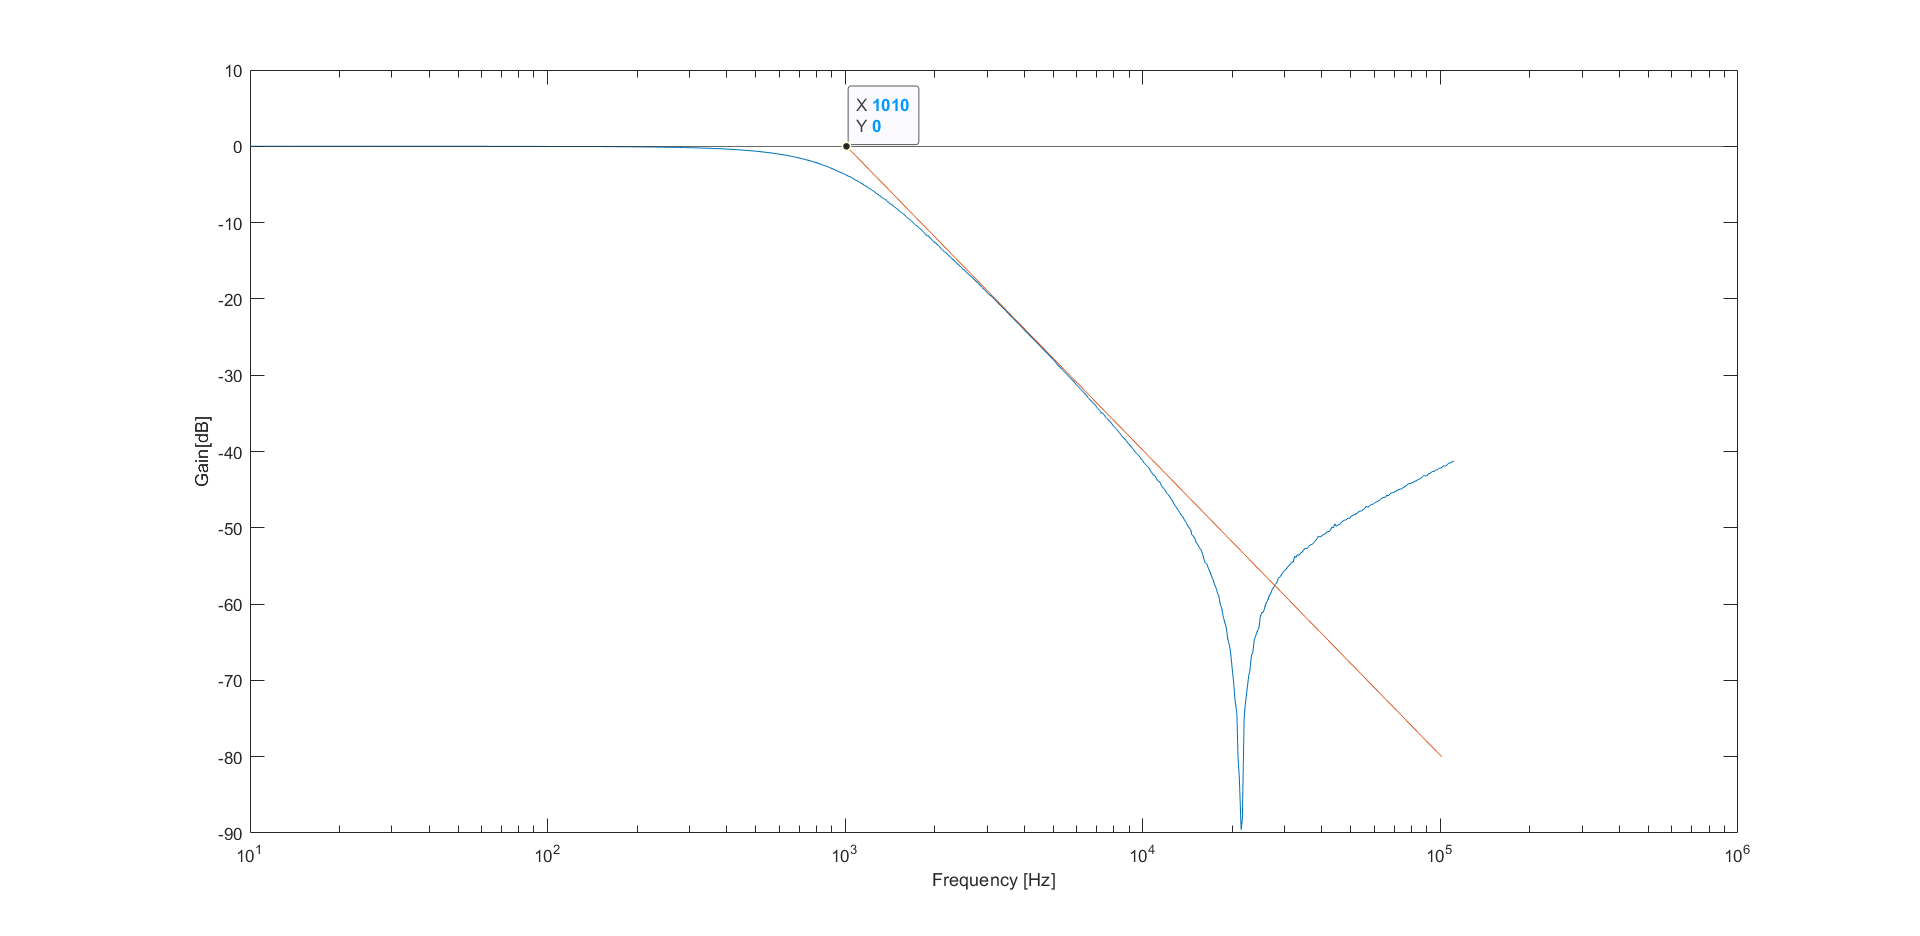
\includegraphics[width=14cm]{2ratio2.png}
    \caption{$C_1/C_2$ $\approx$ 2}
    \label{fig:my_label}
\end{figure}

A visible peak in the graph (figure 4) displays the effects of the quality factor.

\begin{figure}[h!]
    \centering
    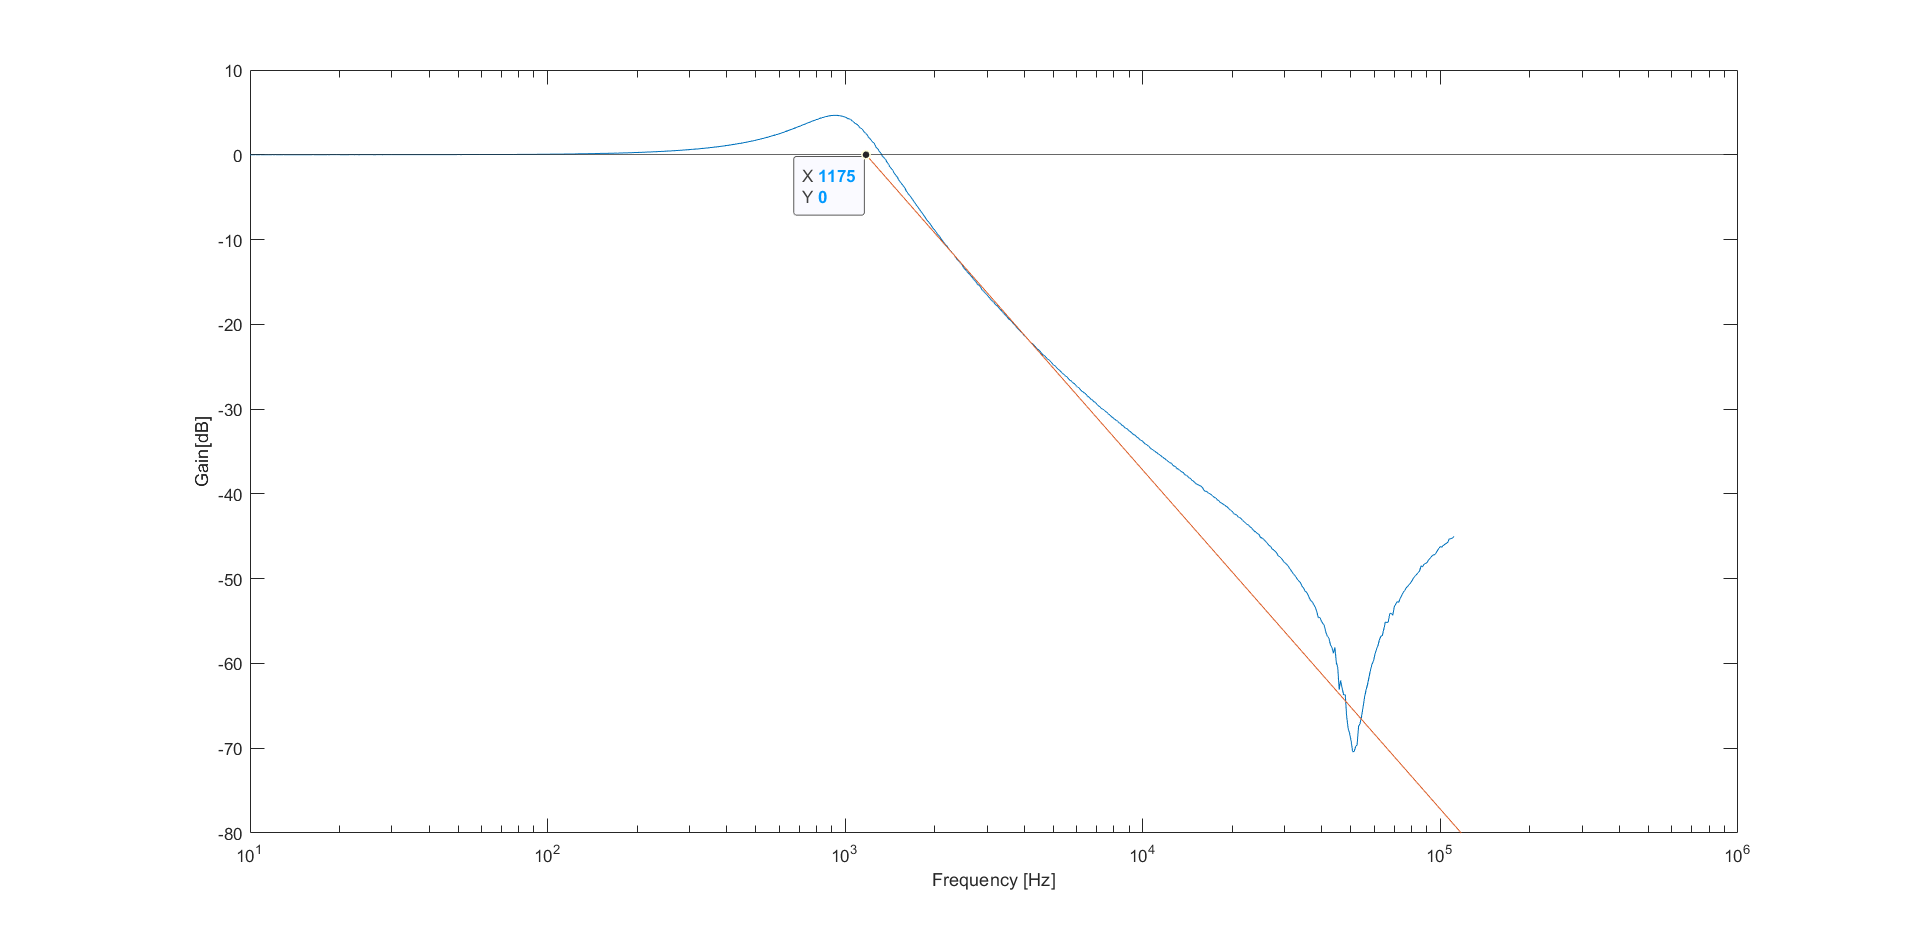
\includegraphics[width=14cm]{20ratio20.png}
    \caption{$C_1/C_2$ $\approx$ 20}
    \label{fig:my_label}
\end{figure}
%Spurning um að sleppa því að mæla/reikna gain??
%Bera saman niðurstöður mælinga og útreikninga \newline
%Benda á skekkjur  \newline
%STATE THE OBVIOUS

%taka út subsections í results???

%\subsection{Sallen-key Circuit}
%Bera saman niðurstöður mælinga og útreikninga \newline
%Benda á skekkjur  \newline
%STATE THE OBVIOUS
\section{Summary}

\subsection{Cascaded Circuit}
%Útskýra mun á mældum niðurstöðum og reiknuðum niðurstöðum.  \newline
%Tho. nálgun er greinilega ekki nógu góð  \newline
The discrepancy between the theoretical and measured value of the cutoff frequency is minimal as the error is only $0.4\%$. It can therefore be deducted that the cutoff frequency does indeed occur when the magnitude of the transfer function drops to $70.71\%$ of its maximum value.

\subsection{Sallen-key Circuit}
%Skoða útleiðslur á quality factor  \newline
%hvaða áhrif hefur quality factor á cut-off frequency? Útleiðslur í bókinni  \newline
%Tengja áhrif transfer function við í rás (hvað er takmarkandi og hvernig)

From the output signals of the Sallen-Key filter it can be observed that the quality factor, Q, affects the sharpness of the peak at the cutoff frequency, the higher the quality factor, the sharper the peak is. The quality factor also directly affects the gain of the circuit as can be observed as well. Also note that the ratio between capacitors greatly affected the quality factor.


\newpage
\appendix
\section{}

    \begin{figure}[H]
    \begin{center}
    \centering
     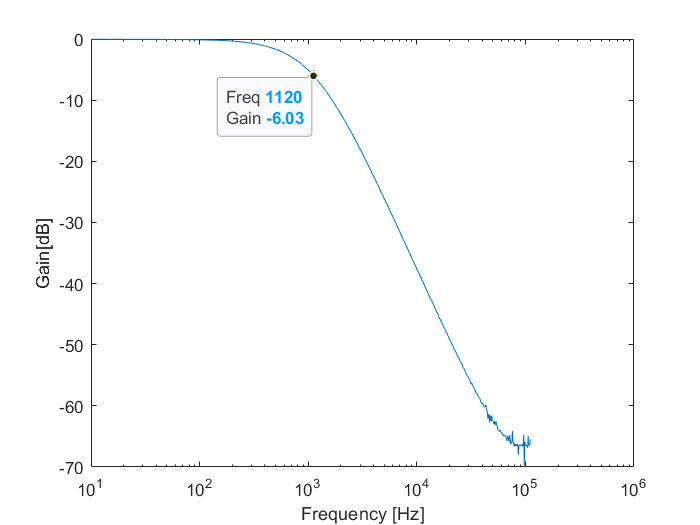
\includegraphics[width=0.9\textwidth]{Task1bodegainplot.png}
     \caption{Task 1}
     \label{distorted_signal}
     \end{center}
     \end{figure}

\end{document}
